\section{Transformation rules (smoothening, scales and shifts).}
As we seen, the Euclidean distance is efficient and easily computable but it doesn't capture similar time-series in the presence of noise, scales or shifts. Many research was done to overcome this issue. In \cite{citeulike:3815880} authors introduced scale and the shift shape-persieving transformations which applied before measuring the similarity with Euclidean distance, their proposed definition of similar time-series based on the similarity transformation $T_{a,b}$ where $a$ is the scaling coefficient and $b$ is the shift coefficient. This ``similarity transformation $T_{a,b}$'' is a mapping of each of the $x_{i} \in X$ into $x_{i}\acute{} = a*x_{i}+b$ and if this transformation can be found for two time-series $X$ and $Y$ such that $X=T_{a,b}(Y)$ time-series $X$ and $Y$ are similar.

Agrawal et al. \cite{citeulike:3816327} proposed a similar method of aligning of time-series but allowing any arbitrary segment of the query time-series to be scaled and stretched by any suitable amount and adding the ability of deletion of any non-matching segment (this work in fact seems to be the one of the first proposing LCS application to time-series similarity, see later). Also they introduced an $\epsilon$ envelope around the template sequence which aimed to deal with noise on the query time-series. The figure  \ref{fig:transform} shows principles of such a method walking from the raw time series through discussed transformations.

\begin{figure}[tbp]
   \centering
   \includegraphics[height=50mm]{transform.eps}
   %%{seriesheatmap}
   \caption{Illustration of the scaling, smoothening and shifting: the leftmost plot depicts the raw time-series, plot at the middle shows the query time-series after scaling and smoothening and the plot at the right adds shifts to transform while showing $\epsilon$ alignment envelope.}
   \label{fig:transform}
\end{figure} 

Each of the transformation is associated with the effective cost .

